\section{jobantechnikteil}
\abschnittsautor{J. Rahal}

\subsection{Gesamtarchitektur und Technologieentscheidungen}

VerTex ist als Drei-Schichten-System aufgebaut (siehe 
Abschnitt~\ref{sec:systemarchitektur}):
Die Datenhaltung übernimmt eine
MariaDB-Datenbank, die Logik ein in Python umgesetztes Backend mit FastAPI und
die Darstellung eine Weboberfläche mit Vue.js. Die Schichten kommunizieren
ausschließlich über die REST-Schnittstelle des Backends, die Daten werden als
JSON ausgetauscht. Umgesetzt wurde von unten nach oben: zuerst die Datenbank,
dann die API, zuletzt die Oberfläche. Eine Oberfläche ohne Daten wäre nur eine
leere Hülle, und die API lässt sich mit Testdaten prüfen, ohne dass die
Bildverarbeitung fertig sein muss.

Für die Datenhaltung fiel die Wahl auf MariaDB, da die Spiel-, Kader- und
Ereignisdaten klar strukturiert sind und sich über Fremdschlüssel widerspruchsfrei
verknüpfen lassen. Im Backend kommt Python mit FastAPI zum Einsatz, weil auch
die Bildverarbeitung in Python umgesetzt wird und FastAPI durch Pydantic eine
automatische Prüfung eingehender JSON-Daten sowie eine interaktive
Schnittstellendokumentation bietet. Für die Weboberfläche wurde Vue.js mit Vite
gewählt, da sich reaktive Komponenten wie das Spielfeld, die Spielauswahl und
die Detailansichten übersichtlich trennen und ohne lange Ladezeiten entwickeln
lassen.

\subsection{Datenbankentwurf und Datenimport}
\label{sec:datenbankentwurf}

Die Datenbank \texttt{vertex} bildet Mannschaften, Spieler, Spiele,
Videoreferenzen, Positionsdaten, Spielereignisse sowie externe Referenzprofile
in acht relationalen Tabellen ab. Den Zusammenhang aller Entitäten und
Fremdschlüssel zeigt das Entity-Relationship-Diagramm in
Abbildung~\ref{fig:er-modell}.


\begin{figure}[htbp]
    \centering
    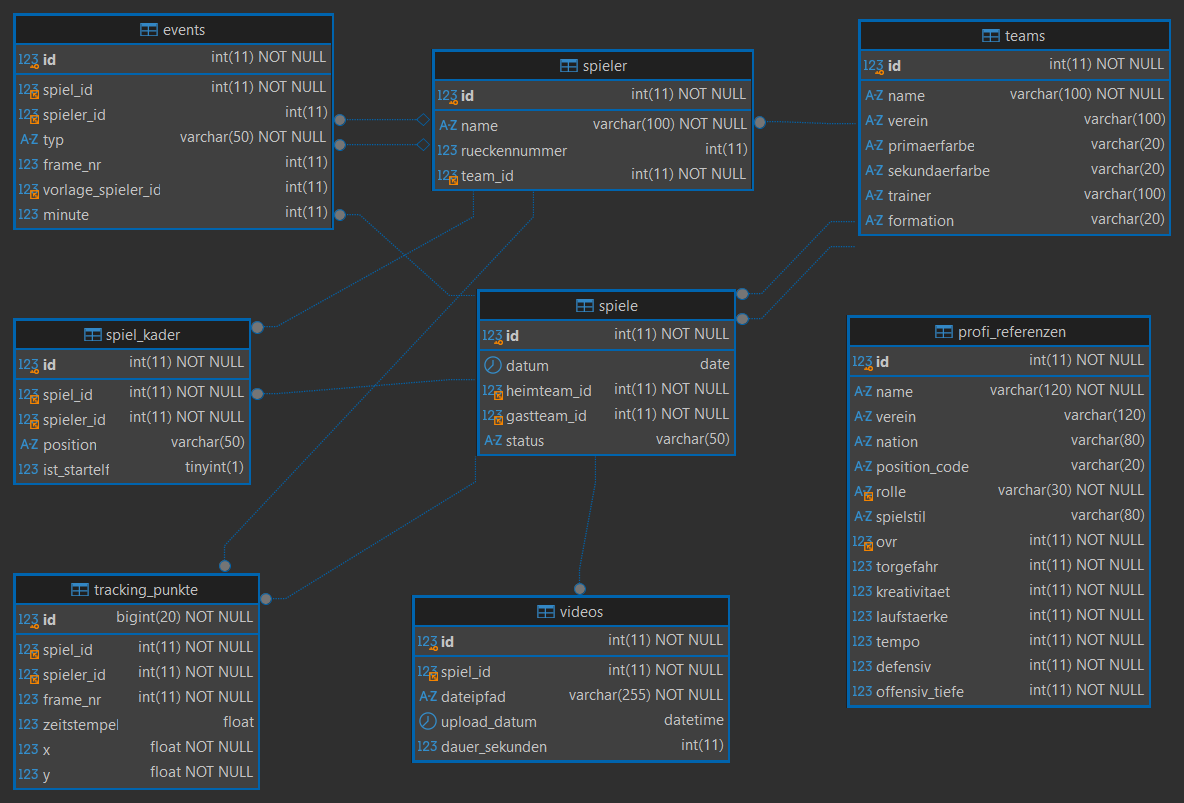
\includegraphics[width=0.95\textwidth]{images/er-modell.png}
    \caption{Relationales Datenbankschema der VerTex-Datenbank in DBeaver.}
    \label{fig:er-modell}
\end{figure}



\begin{itemize}
    \item \texttt{teams}: Speichert Stammdaten jeder Mannschaft (\texttt{name},
    \texttt{verein}) sowie Darstellungs- und Taktikangaben
    (\texttt{primaerfarbe}, \texttt{sekundaerfarbe}, \texttt{trainer},
    \texttt{formation}).
    \item \texttt{spieler}: Enthält alle Spieler mit \texttt{name},
    \texttt{rueckennummer} und dem Fremdschlüssel \texttt{team\_id} auf die
    zugehörige Mannschaft.
    \item \texttt{spiele}: Verwaltet angesetzte und analysierte Begegnungen mit
    \texttt{datum}, \texttt{status} sowie zwei Fremdschlüsseln
    (\texttt{heimteam\_id} und \texttt{gastteam\_id}) auf \texttt{teams}. Das
    Endergebnis wird bewusst nicht redundant gespeichert, sondern zur Laufzeit
    aus den Tor-Ereignissen berechnet.
    \item \texttt{spiel\_kader}: Löst die n:m-Beziehung zwischen Spielen und
    Spielern auf (siehe Abschnitt~\ref{sec:er-modell}). Neben \texttt{spiel\_id}
    und \texttt{spieler\_id} speichert die Tabelle die konkrete
    \texttt{position} im jeweiligen Spiel sowie das Kennzeichen
    \texttt{ist\_startelf} zur Trennung von Startelf und Ersatzbank.
    \item \texttt{videos}: Verknüpft die zu einem Spiel hochgeladenen
    Videoaufnahmen über \texttt{spiel\_id} mit der Tabelle \texttt{spiele} und
    speichert Metadaten wie \texttt{dateipfad}, \texttt{upload\_datum} und
    \texttt{dauer\_sekunden} für die Weiterverarbeitung in der Bildanalyse.
    \item \texttt{tracking\_punkte}: Nimmt die zeitlich aufgelösten
    Spielfeldkoordinaten (\texttt{x}, \texttt{y} in Metern auf einem
    $105 \times 68$\,m großen Feld) pro \texttt{frame\_nr} und
    \texttt{zeitstempel} auf. Aufgrund des hohen Datenvolumens wird für den
    Primärschlüssel der Datentyp \texttt{BIGINT} verwendet.
    \item \texttt{events}: Protokolliert Spielereignisse wie Tore, Schüsse,
    Fouls, Karten und Verletzungen über \texttt{typ}, \texttt{frame\_nr} und
    \texttt{minute}. Ein optionaler zweiter Fremdschlüssel
    \texttt{vorlage\_spieler\_id} verknüpft bei einem Tor zusätzlich den
    Vorlagengeber.
    \item \texttt{profi\_referenzen}: Enthält externe Vergleichsdaten aus einem
    EA-FC-Spielerdatensatz mit Position, Rolle, Spielstil und sechs normierten
    Leistungsattributen für die Spielerprofil-Analyse. Die Tabelle steht
    bewusst ohne Fremdschlüsselbezug als eigenständige Referenztabelle im
    Schema, da die Ähnlichkeit dynamisch zur Laufzeit berechnet wird und sich
    die Zuordnung eines Spielers nach jedem neuen Spiel verändern kann.
\end{itemize}

Da bei einer Bildrate von 25 Bildern pro Sekunde bereits wenige Minuten
Spieldauer mehrere zehntausend Datensätze in \texttt{tracking\_punkte} erzeugen,
führten ungefilterte Abfragen im ersten Prototyp zu spürbaren Ladezeiten im
Frontend. Durch das Anlegen eines zusammengesetzten Index
\texttt{idx\_tracking\_spiel\_spieler} über die Spalten \texttt{spiel\_id} und
\texttt{spieler\_id} liest MariaDB die Laufwege eines einzelnen Spielers gezielt
aus, ohne die gesamte Tabelle durchsuchen zu müssen. Zusätzliche Indizes auf
\texttt{rolle} und \texttt{ovr} in \texttt{profi\_referenzen} beschleunigen den
späteren Attributvergleich.

Um Backend und Oberfläche unabhängig vom Fortschritt der Bildverarbeitung
entwickeln und testen zu können, wurde ein eigenes Python-Skript
(\texttt{simulator.py}) umgesetzt. Es erzeugt für alle abgeschlossenen Spiele
formationsabhängige Kader, realitätsnahe Laufwege mit Jogging- und
Sprintphasen sowie konsistente Spielereignisse, bei denen jedes Tor zugleich
als Schuss gezählt wird. Ersatzspieler bewegen sich lediglich im Bereich der
Seitenlinie, sodass realistische Distanzunterschiede entstehen. Spiele mit dem
Status \texttt{geplant} werden übersprungen und dienen als Datengrundlage für
die Vorschau- und Direktvergleichsansicht. Das Einfügen der Tracking-Punkte
erfolgt paketweise in Blöcken zu je 5\,000 Zeilen, um Speicher- und
Paketgrößenlimits der Datenbank einzuhalten.

Für die Ähnlichkeitsanalyse wurden reale Profidaten über das Skript
\texttt{import\_eafc.py} aus einer CSV-Datei mit 9\,962 Einträgen eingelesen.
Dabei filtert das Skript doppelte Sonderkarten heraus, beschränkt sich auf
aktive Basiskarten ab einer Gesamtwertung von 75 und ordnet die detaillierten
Positionskürzel den vier Grundrollen Torwart, Abwehr, Mittelfeld und Sturm zu.
Insgesamt wurden 2\,525 eindeutige Referenzprofile in \texttt{profi\_referenzen}
gespeichert.

\subsection{Backend und REST-Schnittstelle}
\label{sec:backend}

Das Backend bildet die Logikschicht von VerTex und ist vollständig in
\texttt{main.py} mit dem Python-Framework FastAPI umgesetzt. Die Verbindung zur
MariaDB-Datenbank erfolgt über SQLAlchemy (\texttt{create\_engine}) in
Kombination mit dem Treiber PyMySQL. Zugangsdaten wie Benutzername, Passwort,
Host und Datenbankname werden nicht direkt im Quellcode hinterlegt, sondern
beim Start über \texttt{python-dotenv} aus einer lokalen \texttt{.env}-Datei
geladen. Dadurch bleiben sensible Konfigurationsdaten von der
Versionsverwaltung getrennt.

Da das Vue-Frontend während der Entwicklung auf einem anderen Port
(\texttt{localhost:5173}) läuft als der Backend-Server (\texttt{localhost:8000}),
wurde im Backend die \texttt{CORSMiddleware} von FastAPI aktiviert. Sie gibt
Zugriffe vom Frontend-Ursprung explizit frei, sodass der Browser die
asynchronen HTTP-Anfragen nicht blockiert.

Alle Funktionen des Backends sind als REST-Endpunkte organisiert und liefern
ihre Ergebnisse im JSON-Format zurück. Tabelle~\ref{tab:api-endpunkte} gibt
einen Überblick über die implementierten Schnittstellen.

\begin{table}[htbp]
    \centering
    \footnotesize
    \caption{Übersicht der implementierten REST-Endpunkte des VerTex-Backends.}
    \label{tab:api-endpunkte}
    \begin{tabular}{l p{5.8cm} p{6.2cm}}
        \hline
        \textbf{Methode} & \textbf{Pfad} & \textbf{Aufgabe} \\
        \hline
        \texttt{GET} & \texttt{/api/teams} &
        Liefert alle Mannschaften inklusive Teamfarben, Trainer und Grundformation. \\
        \texttt{GET} & \texttt{/api/matches} &
        Liefert alle Spiele mit dynamisch berechneten Spielständen und Zukunftskennzeichen. \\
        \texttt{GET} & \texttt{/api/matches/\{match\_id\}/players} &
        Lädt Startelf und Ersatzbank eines Spiels samt Positionen und Rückennummern. \\
        \texttt{GET} & \texttt{/api/matches/\{match\_id\}/events} &
        Gibt alle Spielereignisse (Tore inkl.\ Vorlagengeber, Karten, Verletzungen, Schüsse) chronologisch aus. \\
        \texttt{GET} & \texttt{/api/matches/\{match\_id\}/tracking} &
        Liefert Positionsdaten eines Spiels, optional per Query-Parameter \texttt{spieler\_id} auf einen Spieler gefiltert. \\
        \texttt{GET} & \texttt{/api/matches/\{match\_id\}/h2h} &
        Berechnet die Direktvergleichs-Historie sowie die Team- und Trainer-Erfolgsquoten. \\
        \texttt{GET} & \texttt{/api/standings} &
        Erstellt die aktuelle Liga-Tabelle aus allen abgeschlossenen Partien. \\
        \texttt{GET} & \texttt{/api/players/\{spieler\_id\}/profile} &
        Erzeugt das sechsdimensionale Spielerprofil und berechnet das EA-FC-Ähnlichkeitsmatch. \\
        \texttt{POST} & \texttt{/api/matches/\{match\_id\}/ingest} &
        Nimmt Tracking- und Ereignisdaten der Bildverarbeitung entgegen und speichert sie transaktional. \\
        \hline
    \end{tabular}
\end{table}

Eine zentrale Rolle für die Zusammenarbeit im Projektteam spielt der Endpunkt
\texttt{POST /api/matches/\{match\_id\}/ingest}. Statt direkt auf die Datenbank
zuzugreifen, übermitteln die Module der Bildverarbeitung ihre Ergebnisse als
strukturiertes JSON-Objekt an diese Schnittstelle. FastAPI prüft die eingehende
Nutzlast mithilfe der Pydantic-Modelle \texttt{TrackingPunkt}, \texttt{EventIn}
und \texttt{MatchIngestPayload} automatisch auf vollständige Felder und korrekte
Datentypen; fehlerhafte Anfragen werden direkt mit dem HTTP-Statuscode 422
abgewiesen. Listing~\ref{lst:ingest-json} zeigt die erwartete JSON-Struktur.

\begin{figure}[htbp]
    \centering
    \begin{minipage}{0.92\textwidth}
\begin{verbatim}
{
  "status": "analysiert",
  "tracking": [
    { "spieler_id": 9, "frame_nr": 1, "zeitstempel": 0.04, "x": 54.2, "y": 33.8 }
  ],
  "events": [
    { "spieler_id": 9, "vorlage_spieler_id": 10, "typ": "Tor", "frame_nr": 1420, "minute": 34 },
    { "spieler_id": 4, "typ": "Gelbe Karte", "frame_nr": 2100, "minute": 61 }
  ]
}
\end{verbatim}
    \end{minipage}
    \caption{JSON-Datenformat für den Import von Analyseergebnissen über den Ingest-Endpunkt.}
    \label{lst:ingest-json}
\end{figure}

Beim Speichern öffnet SQLAlchemy über \texttt{engine.begin()} eine atomare
Datenbanktransaktion. Bereits vorhandene Daten desselben Spiels werden ersetzt,
neue Positionsdaten paketweise in Blöcken zu je 5\,000 Zeilen eingefügt und der
Spielstatus abschließend auf \texttt{analysiert} gesetzt. Tritt während des
Schreibvorgangs ein Fehler auf, wird die gesamte Transaktion zurückgerollt,
sodass keine unvollständigen Spieldaten entstehen. Über die von FastAPI
automatisch generierte Swagger-Oberfläche unter \texttt{/docs} lässt sich diese
Schnittstelle ohne zusätzlichen Client direkt im Browser testen.

Neben dem reinen Lesen und Schreiben übernimmt das Backend mehrere
Auswertungen direkt serverseitig. Bei \texttt{GET /api/matches} ermittelt eine
SQL-Unterabfrage den Spielstand aus den Tor-Ereignissen beider Teams und setzt
über einen Vergleich mit dem Tagesdatum sowie dem Spielstatus das Feld
\texttt{ist\_zukunft}. Der Endpunkt \texttt{GET /api/standings} aggregiert aus
allen abgeschlossenen Partien Siege, Unentschieden, Niederlagen, Tordifferenz,
Punkte und die prozentuale Erfolgsquote und sortiert die Tabelle nach Punkten,
Tordifferenz und erzielten Toren. Für die Spielvorschau berechnet
\texttt{GET /api/matches/\{match\_id\}/h2h} sowohl die Bilanz aller bisherigen
direkten Duelle beider Mannschaften als auch die Saisonbilanz, den Punkteschnitt
und die Formkurve der letzten fünf Spiele pro Team und Trainer. Die algorithmische
Berechnung des Spielerprofils und des Profi-Vergleichs unter
\texttt{/api/players/\{spieler\_id\}/profile} wird im folgenden Abschnitt im
Detail beschrieben.

\subsection{Spielerprofil- und Ähnlichkeitsanalyse}
\label{sec:spielerprofil}

Über den Endpunkt \texttt{GET /api/players/\{spieler\_id\}/profile} erstellt
das Backend für jeden Spieler ein quantitatives Leistungsprofil und ordnet
dieses dem ähnlichsten Referenzprofil aus der Tabelle
\texttt{profi\_referenzen} zu. Dabei trennt die API sauber zwischen den
spielbezogenen Kennzahlen (\texttt{spiel\_stats}), die exakt zum ausgewählten
Spielstand passen, und den saisonübergreifenden Gesamtwerten
(\texttt{saison\_stats}), aus denen ein stabileres Spielstilprofil abgeleitet
wird.

\subsubsection{Extraktion von Bewegungs- und Ereigniskennzahlen}

Aus den chronologisch sortierten Koordinaten $(x_i, y_i)$ eines Spielers in
\texttt{tracking\_punkte} berechnet das Backend zunächst die zurückgelegte
Laufdistanz $D$ in Metern als Summe der euklidischen Abstände zwischen
aufeinanderfolgenden Einzelbildern:

\begin{equation}
    D = \sum_{i=1}^{N-1} \sqrt{(x_i - x_{i-1})^2 + (y_i - y_{i-1})^2}
    \label{eq:laufdistanz}
\end{equation}

Für jedes Bildintervall $\Delta t_i = t_i - t_{i-1}$ (bei 25 Bildern pro
Sekunde entspricht dies standardmäßig $0{,}04\,\mathrm{s}$) wird die
Momentangeschwindigkeit $v_i = d_i / \Delta t_i$ bestimmt und zur Unterdrückung
möglicher Tracking-Ausreißer auf maximal $10{,}6\,\mathrm{m/s}$ begrenzt. Da
einzelne Messspitzen die reale Sprintleistung verzerren können, wird die
Spitzengeschwindigkeit $v_{\max}$ nicht über das absolute Maximum, sondern über
das 99.~Perzentil der Geschwindigkeitsverteilung ermittelt und in
$\mathrm{km/h}$ umgerechnet ($v_{\max} = v_{99} \cdot 3{,}6$). Ergänzend werden
die mittlere Laufgeschwindigkeit $\bar{v} = D / (N \cdot 0{,}04)$ sowie die
durchschnittliche Offensiv-Tiefe $\bar{x}_{\mathrm{norm}} \in [0, 100]$
berechnet. Um Heim- und Gastmannschaft vergleichbar zu machen, wird die
$x$-Koordinate der Gastmannschaft vor der Mittelwertbildung an der Feldlänge
von $105\,\mathrm{m}$ gespiegelt ($x' = 105 - x$).

\subsubsection{Abbildung auf den sechsdimensionalen Attributvektor}

Um die erfassten Spiel- und Bewegungsdaten mit den externen EA-FC-Referenzdaten
vergleichbar zu machen, werden die Rohwerte in einen sechsdimensionalen
Attributvektor $\vec{u} = (u_1, u_2, u_3, u_4, u_5, u_6)$ auf einer
Skala von 0 bis 99 überführt. Die sechs Dimensionen repräsentieren
\textit{Torgefahr}, \textit{Kreativität}, \textit{Laufstärke}, \textit{Tempo},
\textit{Defensivarbeit} und \textit{Offensivdrang}.

Für die Ableitung der Geschwindigkeit in den Tempowert $u_4$ wird eine lineare
Skalierung verwendet, die realistische Fußball-Sprintwerte abbildet:

\begin{equation}
    u_4 = \min\Big(99,\; \max\big(30,\; 35 + 3{,}8 \cdot (v_{\max} - 20{,}0)\big)\Big)
    \label{eq:pace-skalierung}
\end{equation}

Eine Geschwindigkeit von $20{,}0\,\mathrm{km/h}$ entspricht damit einem
Tempowert von 35, $31{,}0\,\mathrm{km/h}$ einem Wert von 77 und
$35{,}0\,\mathrm{km/h}$ einem Spitzenwert von 92. Analog skaliert die
Laufstärke $u_3$ über die mittlere Laufgeschwindigkeit $\bar{v}$ in den Bereich
zwischen 30 und 96. Die ereignisabhängigen Attribute \textit{Torgefahr} ($u_1$),
\textit{Kreativität} ($u_2$) und \textit{Defensivarbeit} ($u_5$) kombinieren
positionsabhängige Grundwerte mit den auf Einsätze normierten Ereignisquoten
(Tore, Schüsse, Vorlagen und Fouls) sowie der mittleren Spielfeldposition. Für
Torhüter gelten angepasste Referenzwerte, da klassische Offensivmetriken auf
dieser Position keine Aussagekraft besitzen.

\subsubsection{Positionsfilterung und Ähnlichkeitsberechnung}

Analog zu modernen Scouting- und Sportanalysesystemen erfolgt vor dem
eigentlichen Vergleich eine strikte Vorfilterung nach der Grundrolle
(\textit{Torwart}, \textit{Abwehr}, \textit{Mittelfeld} oder \textit{Sturm}).
Dadurch werden nur Spieler derselben Positionsgruppe aus den 2\,525 Einträgen
in \texttt{profi\_referenzen} herangezogen und fachlich sinnlose Vergleiche
zwischen verschiedenen Mannschaftsteilen ausgeschlossen.

Für jeden verbliebenen Referenzvektor $\vec{p}$ wird die Ähnlichkeit zu
$\vec{u}$ über eine Kombination zweier Abstandsmaße bestimmt. Die
Kosinus-Ähnlichkeit bewertet die Richtung der Vektoren und erfasst damit, ob
das relative Stärken-Schwächen-Profil (der Spielstil) übereinstimmt:

\begin{equation}
    \mathrm{sim}_{\cos}(\vec{u}, \vec{p}) =
    \frac{\sum_{k=1}^{6} u_k \cdot p_k}
    {\sqrt{\sum_{k=1}^{6} u_k^2} \cdot \sqrt{\sum_{k=1}^{6} p_k^2}}
    \label{eq:cosine}
\end{equation}

Da die Kosinus-Ähnlichkeit gegenüber einer reinen Skalierung der Werte
unempfindlich ist, wird sie um eine gewichtete euklidische Distanz ergänzt, die
auch absolute Niveauunterschiede berücksichtigt:

\begin{equation}
    d_w(\vec{u}, \vec{p}) = \sqrt{\sum_{k=1}^{6} w_k \cdot (u_k - p_k)^2},
    \qquad
    \mathrm{sim}_{\mathrm{dist}}(\vec{u}, \vec{p}) = 1 - \frac{d_w(\vec{u}, \vec{p})}{d_{\max}}
    \label{eq:euklid}
\end{equation}

Der Gewichtungsvektor $\vec{w} = (1{,}3;\; 1{,}2;\; 1{,}0;\; 1{,}1;\; 1{,}3;\; 1{,}2)$
betont dabei vor allem die prägenden Offensiv- und Defensivmerkmale
(\textit{Torgefahr} und \textit{Defensivarbeit}), während
$d_{\max} = \sqrt{\sum_{k=1}^{6} w_k \cdot 99^2} \approx 263{,}79$ die maximal
mögliche Distanz zur Normierung auf das Intervall $[0, 1]$ darstellt. Beide
Komponenten fließen abschließend im Verhältnis 55\,\% zu 45\,\% in den
Gesamtscore ein:

\begin{equation}
    S(\vec{u}, \vec{p}) = \big(0{,}55 \cdot \mathrm{sim}_{\cos}(\vec{u}, \vec{p})
    + 0{,}45 \cdot \mathrm{sim}_{\mathrm{dist}}(\vec{u}, \vec{p})\big) \cdot 100\,\%
    \label{eq:gesamtscore}
\end{equation}

Die Ergebnisse werden absteigend nach $S(\vec{u}, \vec{p})$ sortiert und als
Top-3-Auswahl inklusive Verein, Position, Gesamtwertung und dem aus dem
Datensatz extrahierten FC-IQ-Spielstil an das Frontend übermittelt. Sollte die
Tabelle \texttt{profi\_referenzen} in einer Testumgebung nicht befüllt sein,
greift automatisch ein Fallback auf zehn intern hinterlegte Referenzprofile,
sodass der Endpunkt jederzeit lauffähig bleibt.